\section*{LECTURE 1}
\section{Logistics}
If you haven't checked out these course logistics, here are some useful links.
\begin{itemize}
    \item The course syllabus can be found on Canvas - \url{https://canvas.cmu.edu/files/5927463/download?download_frd=1}.
    \item If you haven't filled out the course survey, please do so here - \url{https://forms.gle/8MW6STDPHENtWH9Z6}. 
    \item Log into the course slack for all course communication - the workspace is \url{16-745optimalcontrol.slack.com}.
    \item Also check out the course github. We’ll be using this for distributing and collecting homeworks from you, and posting lecture notes, etc. \url{https://github.com/Optimal-Control-16-745}.
\end{itemize}

\section{Fundamentals}
We first describe some fundamental concepts that we'll use throughout the course. 

\subsection{Continuous Time Dynamics}
The most general way of describing smooth dynamical systems is via a dynamics function: 
\begin{align}
    \dot{x} &= f(x, u)
\end{align}
Here, $x \in \mathbb{R}^n$ describes the state of the system, $u \in \mathbb{R}^n$ is the control input provided to the system, and $f$, the dynamics function, specifies how the system evolves with the application of control inputs. 
$\dot{x}$ provides the derivatives (with respect to time) of state. \\

\begin{figure}
    \centering
    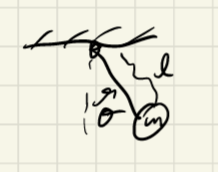
\includegraphics[]{L1_Images/F1.PNG}
    \caption{Simple pendulum system}
    \label{fig:f1}
\end{figure}

\noindent
For a mechanical system, the state $x$ is usually described as:
\begin{align}
    x &= \begin{bmatrix}
            q \\
            v
        \end{bmatrix}
\end{align}
where $q$ describes the configuration of the system, and $v$ describes the velocity. 

\subsubsection{Validity of Assumptions}
Note that the configuration isn't necessarily a vector, and the velocities are not necessarily derivatives of configuration! Also, remember that this description of the system is valid only when the dynamics are smooth. This is broken when, for instance, the system experiences contacts. 

\subsubsection{Example}
Consider the example of a simple pendulum \cref{fig:f1}. The system dynamics can be captured in the following equation: 
\begin{align}
    m l^2 \ddot{\theta} + m g l \sin(\theta) = \tau
\end{align}
Here, the configuration $q$ is given by the pendulum angle $\theta$, the velocity $v$ is specified by $\dot{theta}$, and the control inputs $u$ are given by the torque applied to the system $\tau$.

\noindent
Thus the state $x$ is: 
\begin{align}
    x &= \begin{bmatrix}
            \theta \\
            \dot{\theta} 
        \end{bmatrix}
\end{align} 
The velocity $\dot{x}$ is:
\begin{align}
    \dot{x} &= \begin{bmatrix} 
            \dot{\theta}  \\
            \ddot{\theta} 
        \end{bmatrix}
        = 
        \begin{bmatrix}
            \dot{\theta} \\
            -\frac{q}{l} \sin{\theta} + \frac{1}{m l^2} u
        \end{bmatrix}
\end{align} 
Here, the system dynamics $f(x,u)$ are given as 
\begin{align}
    f(x,u) = 
        \begin{bmatrix}
            \dot{\theta} \\
            -\frac{q}{l} \sin{\theta} + \frac{1}{m l^2} u
        \end{bmatrix}
\end{align} 
The manifold of state here is described as $x \in \mathbb{S}^1 \times \mathbb{R}$, a cylinder.

\subsection{Control-Affine Systems}
Many systems (mechanical systems in particular) can be defined as a \textit{control-affine system}. This is a specific form of the general dynamics described above, where the control inputs affect the system via an affine matrix $G$. 
\begin{align}
    \dot{x} = f_{0} (x) + G(x) u 
\end{align}
For instance, the pendulum system can be described as a control-affine system, where 
\begin{align}
    f_{0}(x) = \begin{bmatrix}
        \dot{\theta} \\
        - \frac{q}{l} \sin(\theta)
    \end{bmatrix}
    \ \ \
    G(x) = \begin{bmatrix}
        0 \\
        \frac{1}{ml^2}
    \end{bmatrix}
\end{align}
In driftless systems, $f_{0}(x)=0$. One can also convert systems to control-affine systems, by adding original control inputs $u$ to state, and setting the modified control inputs (of the control-affine system) to be the derviatives of $u$.

\subsection{Manipulator Dynamics}
Another common form of expressing dynamics is - 
\begin{align}
    M(q) \dot{v} + C(q,u) = B(q) u
\end{align}
Where $M(q)$ is the mass matrix of the system, $C(q,u)$ is the dynamics bias (including Coriolis terms and gravity), and $B(q)$ is the control input jacobian. As usual, $q$  is the configuration and $v$ is the velocity. 
Here, the change in configuration $\dot{q}$:
\begin{align}
    \dot{q} = G(q) v
\end{align}
describe the kinematics of the system.
\begin{align}
    \dot{x} = f(x,u) = \begin{bmatrix}
        G(q) v \\
        -{M(q)}^{-1} ( B(q) u - C ) 
    \end{bmatrix}
\end{align}
In the pendulum system, the mass matrix $M(q) = ml^2$, $C(q,u) = q l \sin(\theta)$, $B=I$, $G=I$.\\

\noindent
All mechanical systems can be described in this form; this is because this form is a different way of expressing the Euler-Lagrange equation for:
\begin{align}
    L = 1/2 \ u^T M(q) u - V(q)
\end{align}

\subsection{Linear Systems}
Linear systems are common way of expressing control problems and designing controllers, since we know how to solve linear systems, and they are relatively simple to deal with. 
\begin{align}
    \dot{x} = A(t) x + B(t) u 
\end{align}
These linear systems are either linearly time invariant, when matrices $A(t)$ and $B(t)$ are constant over time. 
They are linearly time varying systems otherwise. \\

\noindent
We typically approximate non-linear systems with linear systems by linearizing the system around the current state. 
Then - 
\begin{align}
    \dot{x} = f(x,u) 
\end{align}
where $A = \frac{\partial f}{\partial x}$ and $B = \frac{\partial f} {\partial u}$. 

\subsection{Equilibria}
We also want to understand equilibria - i.e. the point where a system will remain at rest. Correspondingly - 
\begin{align}
    \dot{x} = f(x,u) = 0
\end{align}
Algebraically, this is described by roots of the dynamics equation. \\

\begin{figure}
    \centering
    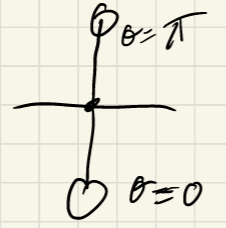
\includegraphics{L1_Images/F2.PNG}
    \caption{Equilibria points of simple pendulum system}
    \label{fig:f2}
\end{figure}


In the pendulum example (without a control input) \cref{fig:f2} - 
\begin{align}
    \dot{x} = \begin{bmatrix}
        \dot{\theta} \\
        -\frac{q}{l} \sin(\theta) 
    \end{bmatrix}
    = 
    \begin{bmatrix}
        0 \\
        0
    \end{bmatrix}
\end{align}
The roots of this occur when $\theta=0$ and $\dot{\theta}=0, \pi$.

\subsubsection{First control problem}
Lets consider a small control problem. Let's try to move the equilibrium point of the pendulum, by applying an appropriate control input. In this case - 
\begin{align}
    \dot{x} = \begin{bmatrix}
        \dot{\theta} \\
        - \frac{q}{l} \sin(\frac{\pi}{2}) + \frac{1}{ml^2} u 
    \end{bmatrix}
    =
    \begin{bmatrix}
        0 \\
        0
    \end{bmatrix}
\end{align}
Solving for $u$, we have:
\begin{align}
    \frac{1}{ml^2} u = - \frac{q}{l} \sin (\frac{\pi}{2}) 
    \implies u = mgl
\end{align}

\subsection{Stability of Equilibria}
We'd also like to understand when a system will return to its equilibrium point upon being perturbed.
Consider a 1-D system, $x \in \mathbb{R}$, as in \cref{fig:f3}.\\

\begin{figure}
    \centering
    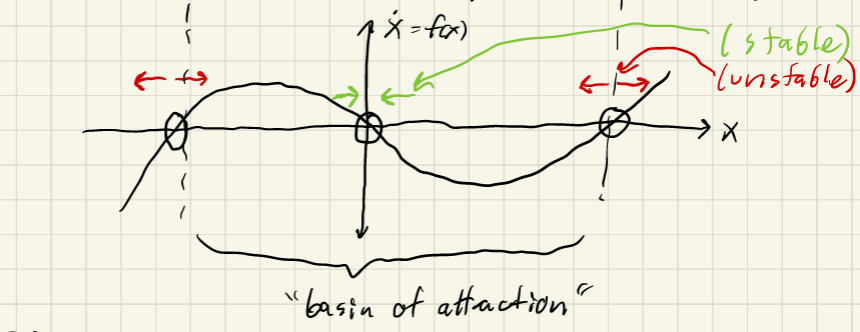
\includegraphics[width=\linewidth]{L1_Images/F3.PNG}
    \caption{Stability of equilibria of a 1-D system.}
    \label{fig:f3}
\end{figure}


\noindent
In this case, when $\frac{\partial f}{\partial x}<0$, the system is stable, because it gets pushed back to the equilibrium point by virtue of the dynamics. Conversely, for $\frac{\partial f}{\partial x}>0$, the system is unstable, because it gets pushed away from the equilibrium point.
The region of $x$ such that  $\frac{\partial f}{\partial x}<0$ is called the basin of attraction of a system.
\\

\noindent
In higher dimensions, $\frac{\partial f}{\partial x}$ is a Jacobian matrix. To study stability of such a system, we can take an Eigen decomposition of the Jacobian (decoupling it into $n$ 1-D systems). If the real-component of each of the eigven values of the Jacobian is less than $0$, the system is stable. Mathematically, the system is stable if
\begin{align}
    \textrm{Re} \big[ eig ( \frac{\partial f}{\partial x} ) \big] < 0 
\end{align}
and unstable otherwise. \\

\noindent
In our pendulum example, 
\begin{align}
    f(x) = \begin{bmatrix}
        \dot{\theta} \\
        - \frac{q}{l} \sin(\theta) 
    \end{bmatrix}
    \implies
    \frac{\partial f}{\partial x} = \begin{bmatrix}
        0 & 1 \\
        - \frac{q}{l} \cos(\theta) & 0
    \end{bmatrix}
\end{align}
Consider the equilibrium point $\theta=\pi$. 
\begin{align}
    \implies
        \evalat{\frac{\partial f}{\partial x}}{\theta=\pi} = \begin{bmatrix}
        0 & 1 \\
        \frac{q}{l} & 0
    \end{bmatrix}
    \implies
    eig(\evalat{\frac{\partial f}{\partial x}}{\theta=\pi}) = \pm \sqrt{\frac{q}{l}}
\end{align}
Since one eigenvalue is negative, the equibilrium point $\theta=\pi$ is unstable.
In contrast, at the equilibrium point $\theta=0$. 
\begin{align}
    \implies
        \evalat{\frac{\partial f}{\partial x}}{\theta=0} = \begin{bmatrix}
        0 & 1 \\
        - \frac{q}{l} & 0
    \end{bmatrix}
    \implies
    eig(\evalat{\frac{\partial f}{\partial x}}{\theta=\pi}) = 0 \pm i \sqrt{\frac{q}{l}}
\end{align}
In this case, the real part of the eigenvalue is $0$. In this purely imaginary eigenvalue case, the system is called marginally stable, and experiences undamped oscillations. 
Adding damping to the systems (such as applying control inputs $u = - K d \dot{\theta}$, results in strictly negative eigenvalues, leading to a stable system. 

\section{References}
Remember to check out \cite{spong2005robot} and \cite{strogatz2016nonlinear} for this course and these topics!

\printbibliography